%%%%%%%%%%%%%%%%%%%%%%%%%%%%%%%%%%%%%%%%%%%%%%%%%%
%%%%%%%%%%%%%%%%%%%%%%%%%%%%%%%%%%%%%%%%%%%%%%%%%%
%%
%% Based one the "beamer-greek-two" template provided 
%% by the Laboratory of Computational Mathematics, 
%% Mathematical Software and Digital Typography, 
%% Department of Mathematics, University of the Aegean
%% (http://myria.math.aegean.gr/labs/dt/)
%%
%% Adapted by Fabian Gröger, June 2020
%%
%%%%%%%%%%%%%%%%%%%%%%%%%%%%%%%%%%%%%%%%%%%%%%%%%%
%%%%%%%%%%%%%%%%%%%%%%%%%%%%%%%%%%%%%%%%%%%%%%%%%%
%%
\PassOptionsToPackage{unicode}{hyperref}
\PassOptionsToPackage{naturalnames}{hyperref}

% to use normal slides ratio
% \documentclass{beamer}

% to use 16:9 ratio
% \documentclass[aspectratio=169, professionalfonts]{beamer} 
\documentclass[aspectratio=169]{beamer}

%\usepackage{babel}
% \usepackage[utf8]{inputenc}

%%% FONT SELECTION %%%%%%%%%%%%%%%%%
%%% sans font %%%%%%%%%%
%\usepackage{kmath,kerkis} %  Font ksf8a at 2160 not found
%\usepackage[default]{gfsneohellenic} 

%%% Times NR %%%%%%%%%%
% \usepackage{newtxtext,newtxmath}
%%%%%%%%%%%%%%%%%%%%%%%%%%%%%%%%%%%%

\usepackage{color}
\usepackage{amsmath}
\usepackage{amssymb}

\usepackage{pgfgantt}
\usepackage{adjustbox}

%\usepackage{media9}
\usepackage{multimedia}

\usepackage{hyperref}
\hypersetup{
    colorlinks=true,
    linkcolor=black,
    filecolor=hslu_pink,      
    urlcolor=hslu_pink,
}

% Have subfigures and captions
\usepackage{subcaption}
\usepackage{caption}

% Tikz to crate diagrams, thanks to: https://github.com/mvoelk/nn_graphics
% Start of tikz settings
\usepackage{tikz}
\usetikzlibrary{positioning,arrows.meta}
\usetikzlibrary{matrix, chains, positioning, decorations.pathreplacing, arrows}
\usetikzlibrary{shapes,arrows,positioning,calc,chains,scopes}

\usepackage{ifthen}
\usepackage{pgfplots}
\pgfplotsset{compat=1.16}
\pgfplotsset{every axis/.append style={tick label style={/pgf/number format/fixed},font=\scriptsize,ylabel near ticks,xlabel near ticks,grid=major}}

\usepackage{amsmath}
\DeclareMathOperator{\sigm}{sigm}
\newcommand{\diff}{\mathop{}\!\mathrm{d}}
\newcommand{\emoji}[1]{\scalerel*{\includegraphics{#1}}{\strut}}
\newcommand{\slidedefault}[3]{\begin{frame}{#1}\begin{columns}[T] \begin{column}{0.8\textwidth}\vbox to .8\textheight{\vfill #2 \vfill}\end{column}\begin{column}{0.2\textwidth}\vbox to .8\textheight{\includegraphics[width=0.75\textwidth]{#3}\vfill}\end{column}\end{columns}\end{frame}}


% colors
\definecolor{snowymint}{HTML}{E3F8D1}
\definecolor{wepeep}{HTML}{FAD2D2}
\definecolor{portafino}{HTML}{F5EE9D}
\definecolor{plum}{HTML}{DCACEF}
\definecolor{sail}{HTML}{A3CEEE}
\definecolor{highland}{HTML}{6D885A}

\tikzstyle{signal}=[arrows={-latex},draw=black,line width=1pt,rounded corners=4pt]

\usepackage{epstopdf}
% \usepackage{graphicx}
\usepackage{graphicx,scalerel}
\graphicspath{{./images/}}

% to make beautiful tables
\usepackage{booktabs}

% appendix for beamer
\usepackage{appendixnumberbeamer}

% notes on beamer template
% when using notes, make sure to have a pdf viewer, which can use the notes
% for example: https://github.com/Cimbali/pympress/
\usepackage{pgfpages}
%\setbeameroption{show notes}
%\setbeameroption{show notes on second screen=right}

%%
% load HSLU thesis layout
\usepackage{HSLU_Thesis_Beamer_Layout}
\setTeipelLayout{}% options: "draft" -> Watermark

\setcounter{tocdepth}{1}
%\beamertemplatenavigationsymbolsempty
\setbeamertemplate{headline}{}

%%%%%%%%%%%%%%%%%%%%%%%%%%%%%%%%%%%%%%%%%%%%%%%%%%%%%%%%%%%%
% Thesis Info %%%%%%%%%%%%%%%%%%%%%%%%%%%%%%%%%%%%%%%%%%%%%%
%%%%%%%%%%%%%%%%%%%%%%%%%%%%%%%%%%%%%%%%%%%%%%%%%%%%%%%%%%%%
	% title
		\title[Master thesis]{Presentation\\ Investigating the Impact of Plant Disease Images on Dermatology Diagnostics}	
	% author
		\author[A. Peter]{Alexander Peter}
	% supervisor
		\supervisor{Supervisor}{Prof. Dr. Marc Pouly, Lucerne University of Applied Sciences and Arts}{Co-Supervisor}{Fabian Gröger, Lucerne University of Applied Sciences and Arts}{Expert}{Tobias Mérinat, Bundesamt für Zoll und Grenzsicherheit}
	% date
		\presentationDate{\today}
%%%%%%%%%%%%%%%%

\begin{document}

% typeset front slides
\typesetFrontSlides

%TODO: consider increasing font size 

%%%%%%%%%%%%%%%%
% Start of Slides:


\slidedefault{Fundamental problem}{
    \begin{itemize}
        \item Public medical data is sparse
        \item Obtaining labelled data is costly
        \item SSL pre-training is sometimes not feasible % Large amount of data for
    \end{itemize}
}{icon_1.png}

\slidedefault{Basic idea}{
    \begin{itemize}
        \item Utilizing data from a similar domain
        \item Considering images of diseased plant leaves
        \begin{tabular}{c c}
            \\
            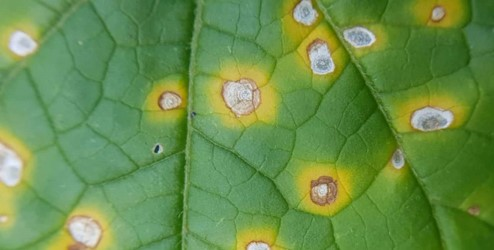
\includegraphics[width=4cm]{spots_on_leaf.jpg} & 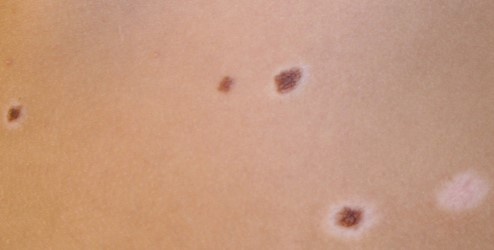
\includegraphics[width=4cm]{sports_on_skin.jpg} \\
        \end{tabular}
    \end{itemize}
}{icon_3.png}

\slidedefault{Method}{
    \framesubtitle{Fine-tuning last layer}
    \begin{itemize}
        \item Last layer during fine tuning
        \item Computationally complex
    \end{itemize}
    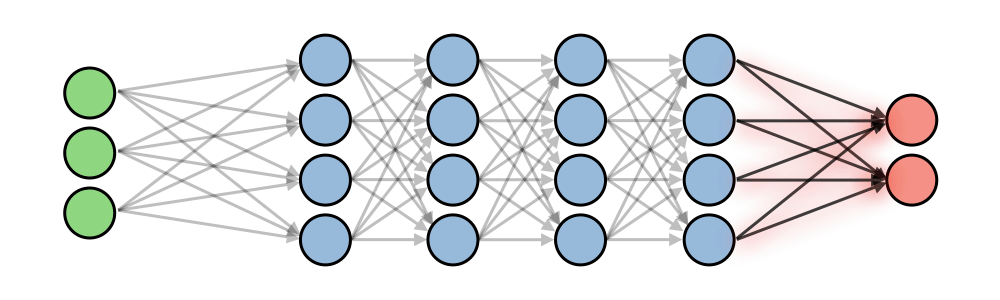
\includegraphics[width=1\textwidth]{fine_tuning_last.png}
}{icon_11.png}

\slidedefault{Method}{
    \framesubtitle{Frozen evaluation}
    \begin{itemize}
        \item Fast algorithms like kNN or linear regression
        \item Reusing features
    \end{itemize}
    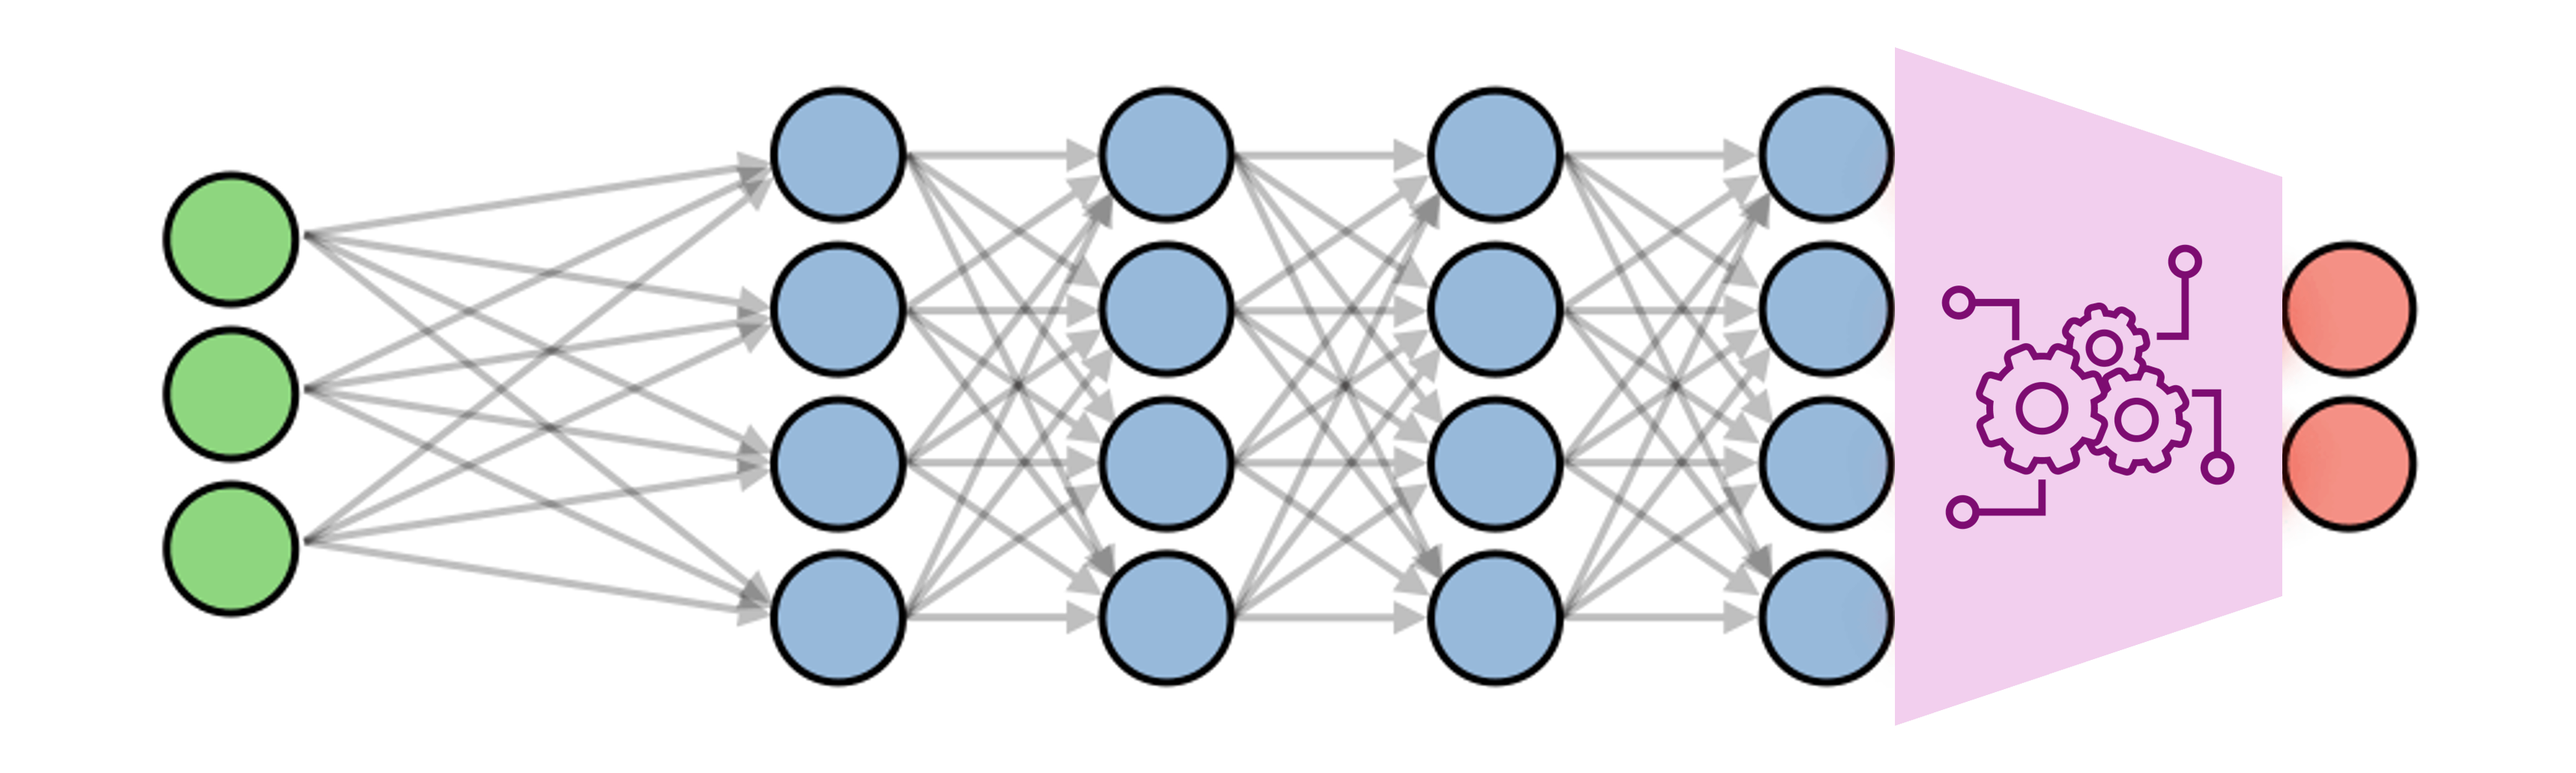
\includegraphics[width=1\textwidth]{frozen_evaluation.png}
}{icon_13.png}

\slidedefault{Expected results}{
    \begin{tabular}{l|c|c}\hline
        \textbf{Pre-training} & \textbf{Plant tasks}  & \textbf{Dermatology tasks} \\\hline
        Random & \emoji{unicode_274c.png} & \emoji{unicode_274c.png} \\\hline
        ImageNet (SSL/SL) & \emoji{unicode_1f949.png} & \emoji{unicode_1f949.png}\\\hline
        Plant (SSL/SL) & \emoji{unicode_1f947.png} & \emoji{unicode_1f948.png} \\\hline
        Dermatology (SSL) & \emoji{unicode_1f948.png} & \emoji{unicode_1f947.png}\\\hline
    \end{tabular}
}{icon_4.png}

\slidedefault{Datasets}{
    \begin{tabular}{c c c c}
        PlantVillage & Cassava & PlantDataset & PlantDoc \\
        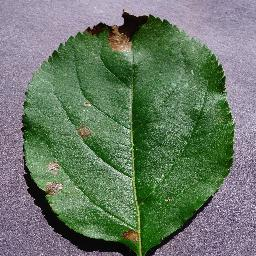
\includegraphics[width=2cm]{sample_plantvillage.jpg} & 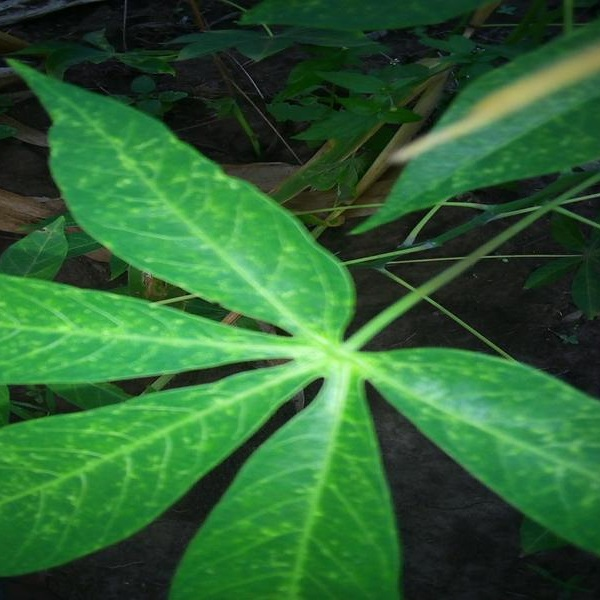
\includegraphics[width=2cm]{sample_cassava.jpg} & 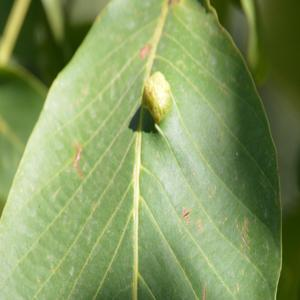
\includegraphics[width=2cm]{sample_plantdataset.jpg} & 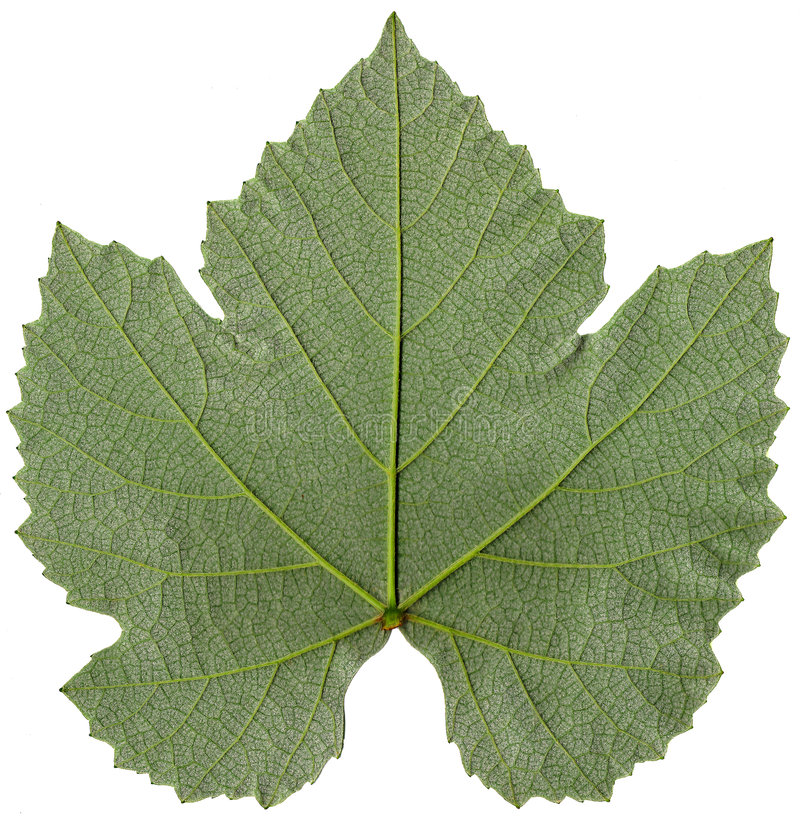
\includegraphics[width=2cm]{sample_plantdoc.jpg} \\
        \\
        DDI & PAD-UFES-20 & HAM10000 & Fitzpatrick17k \\
        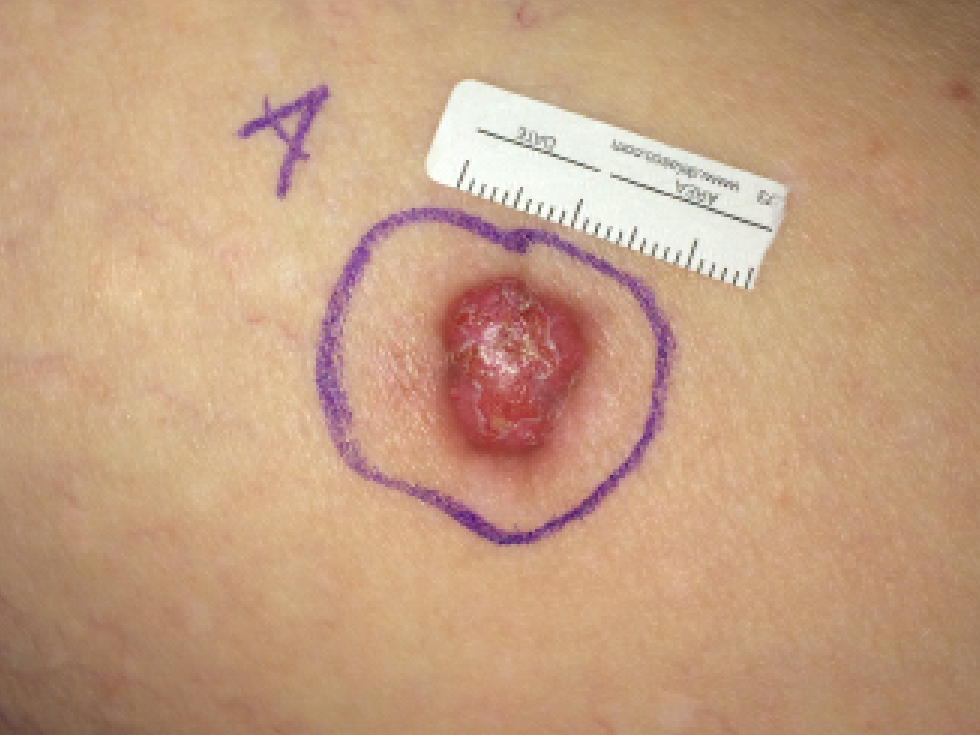
\includegraphics[width=2cm]{sample_ddi.png} & 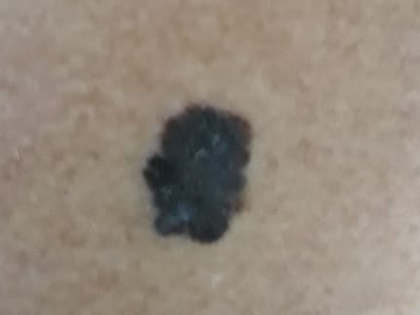
\includegraphics[width=2cm]{sample_padufes20.png} & 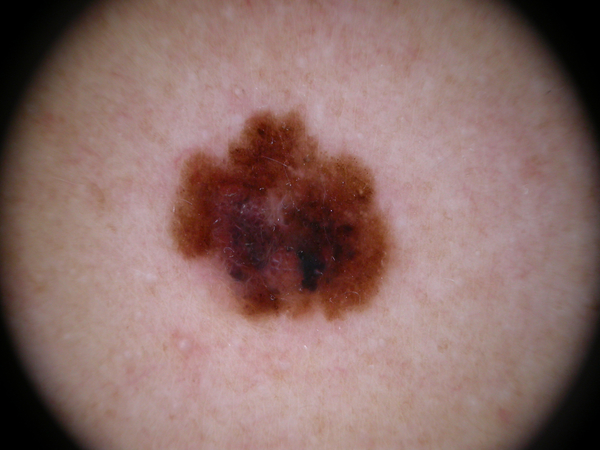
\includegraphics[width=2cm]{sample_ham10000.jpg} & 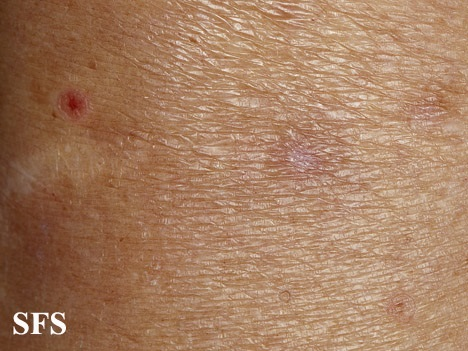
\includegraphics[width=2cm]{sample_fitzpatrick17k.jpg} \\
    \end{tabular}
}{icon_5.png}

\slidedefault{Models \& Weights}{
    \begin{tabular}{|c|c|c|c|c|}\hline
        \multicolumn{1}{|c|}{} & \multicolumn{2}{c|}{\textbf{Resnet50}} & \multicolumn{2}{c|}{\textbf{ViT-T/16}}\\\hline
        & \textbf{SL} & \textbf{SSL} & \textbf{SL} & \textbf{SSL} \\\hline
        \multicolumn{1}{|c|}{Random} & \multicolumn{2}{c|}{Random} & \multicolumn{2}{c|}{Random}\\\hline
        ImageNet & Default & SimCLR & Down-scaled & DINO \\\hline
        Dermatology & -- & SimCLR & -- & DINO \\\hline
        Plant & PDDD & -- & -- & DINO \\\hline
    \end{tabular}
}{icon_7.png}

\slidedefault{Frozen features}{
    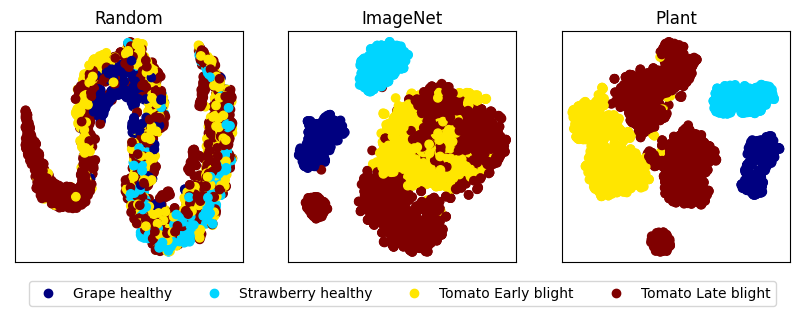
\includegraphics[width=1\textwidth]{features_visualized_with_tsne_combined.png}
    Class similarities within frozen features visualized with t-SNE
}{icon_9.png}

% \textbf{Original} & \textbf{Random} & \textbf{ImageNet} & \textbf{Dermatology} & \textbf{Plant} \\
% 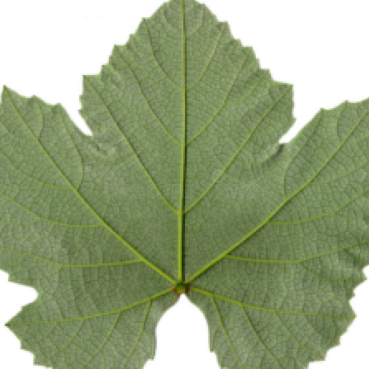
\includegraphics[width=2cm]{attention_input_plantdoc.png} & 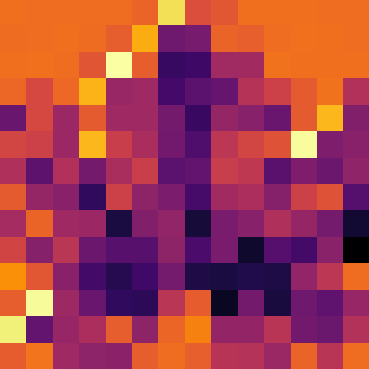
\includegraphics[width=2cm]{attention_ViT_T16-Random_headless_plantdoc.png} & 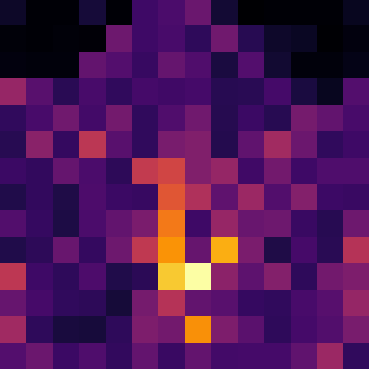
\includegraphics[width=2cm]{attention_ViT_T16-ImageNet_1k_SSL_Dino_headless_plantdoc.png} & 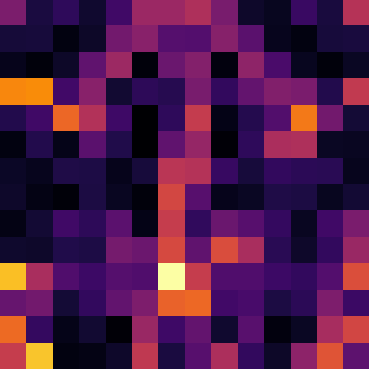
\includegraphics[width=2cm]{attention_ViT_T16-Derma_SSL_Dino_headless_plantdoc.png} & 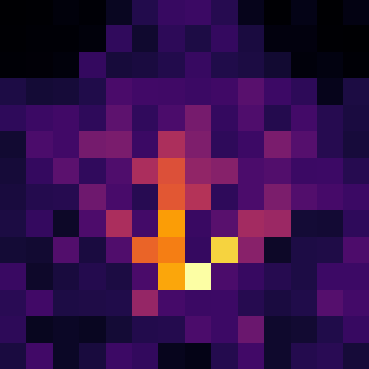
\includegraphics[width=2cm]{attention_ViT_T16-Plant_SSL_Dino_headless_plantdoc.png} \\

\slidedefault{Model attention}{
    \framesubtitle{Random}
    \begin{tabular}{c c c c c}
        \multicolumn{4}{l}{The random model is prone to brightness} \\
        \\
        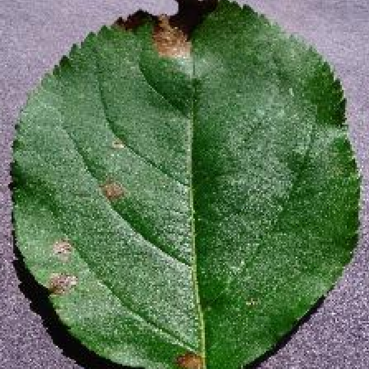
\includegraphics[width=2cm]{attention_input_plantvillage.png} & 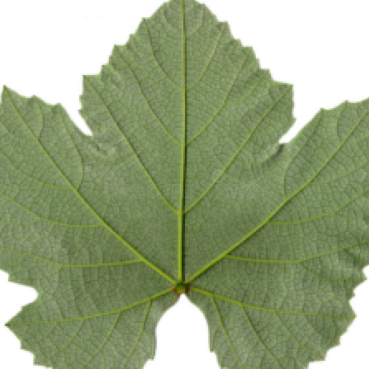
\includegraphics[width=2cm]{attention_input_plantdoc.png} & 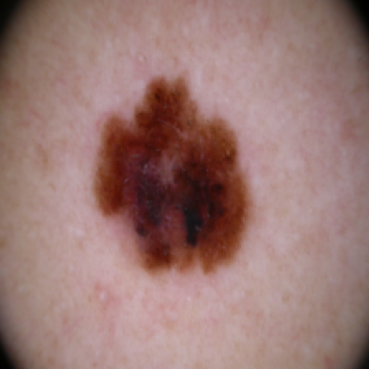
\includegraphics[width=2cm]{attention_input_ham10000.png} & 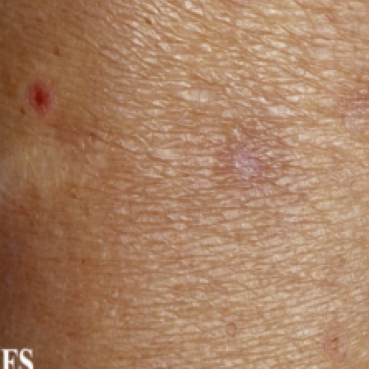
\includegraphics[width=2cm]{attention_input_fitzpatrick17k.png} \\
        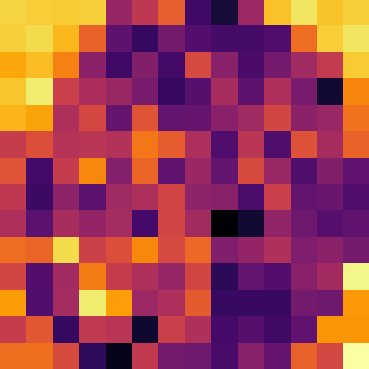
\includegraphics[width=2cm]{attention_ViT_T16-Random_headless_plantvillage.png} & 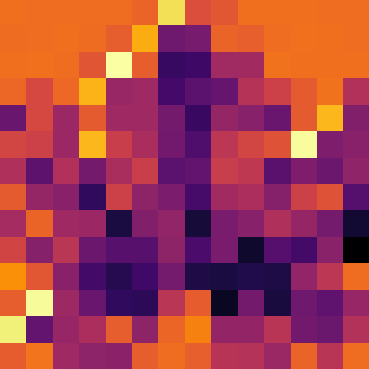
\includegraphics[width=2cm]{attention_ViT_T16-Random_headless_plantdoc.png} & 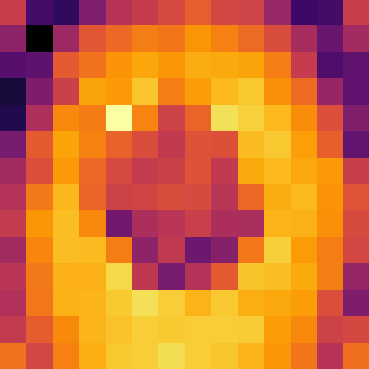
\includegraphics[width=2cm]{attention_ViT_T16-Random_headless_ham10000.png} & 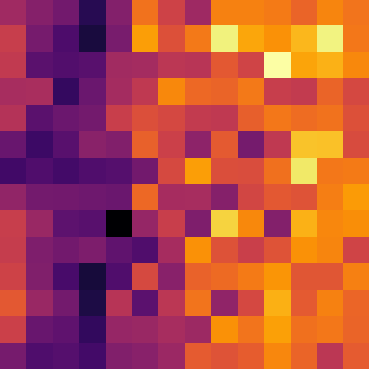
\includegraphics[width=2cm]{attention_ViT_T16-Random_headless_fitzpatrick17k.png} \\
    \end{tabular}
}{icon_8.png}

\slidedefault{Model attention}{
    \framesubtitle{ImageNet}
    \begin{tabular}{c c c c c}
        \multicolumn{4}{l}{The imagenet model mainly focuses on abnormalities} \\
        \\
        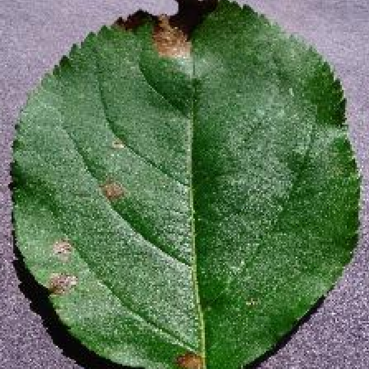
\includegraphics[width=2cm]{attention_input_plantvillage.png} & 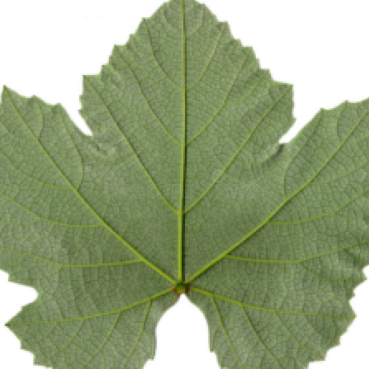
\includegraphics[width=2cm]{attention_input_plantdoc.png} & 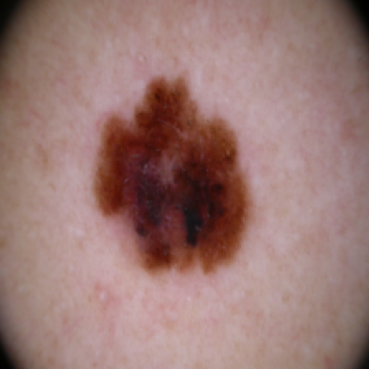
\includegraphics[width=2cm]{attention_input_ham10000.png} & 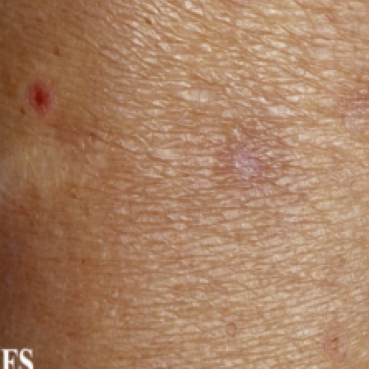
\includegraphics[width=2cm]{attention_input_fitzpatrick17k.png} \\
        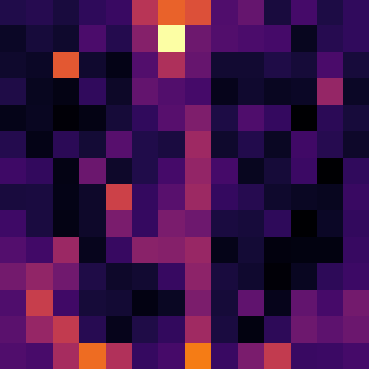
\includegraphics[width=2cm]{attention_ViT_T16-ImageNet_1k_SSL_Dino_headless_plantvillage.png} & 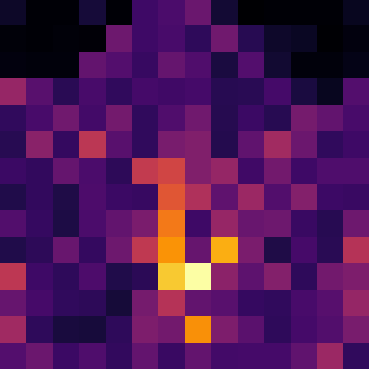
\includegraphics[width=2cm]{attention_ViT_T16-ImageNet_1k_SSL_Dino_headless_plantdoc.png} & 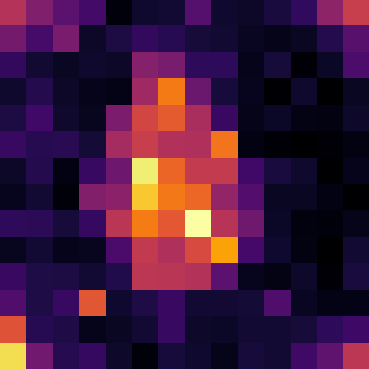
\includegraphics[width=2cm]{attention_ViT_T16-ImageNet_1k_SSL_Dino_headless_ham10000.png} & 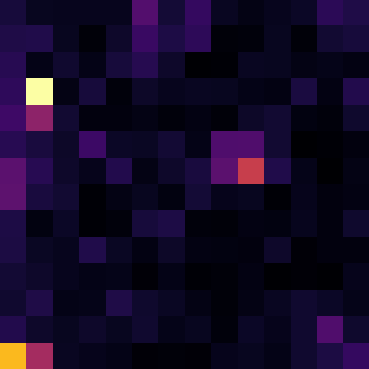
\includegraphics[width=2cm]{attention_ViT_T16-ImageNet_1k_SSL_Dino_headless_fitzpatrick17k.png} \\
    \end{tabular}
}{icon_8.png}

\slidedefault{Model attention}{
    \framesubtitle{Dermatology}
    \begin{tabular}{c c c c c}
        \multicolumn{4}{l}{The dermatology model includes the surrounding area} \\
        \\
        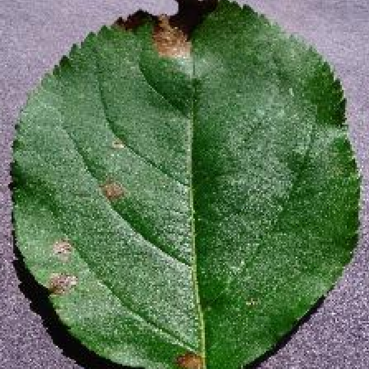
\includegraphics[width=2cm]{attention_input_plantvillage.png} & 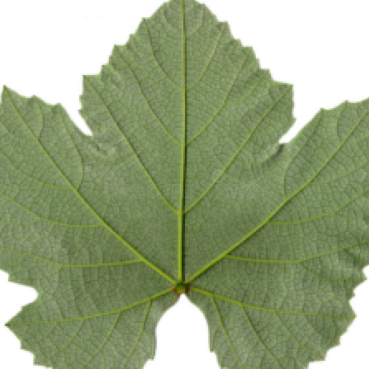
\includegraphics[width=2cm]{attention_input_plantdoc.png} & 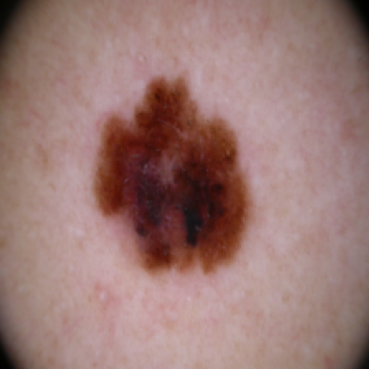
\includegraphics[width=2cm]{attention_input_ham10000.png} & 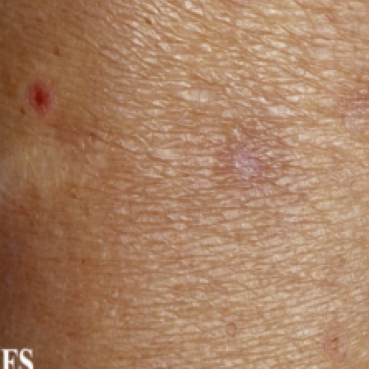
\includegraphics[width=2cm]{attention_input_fitzpatrick17k.png} \\
        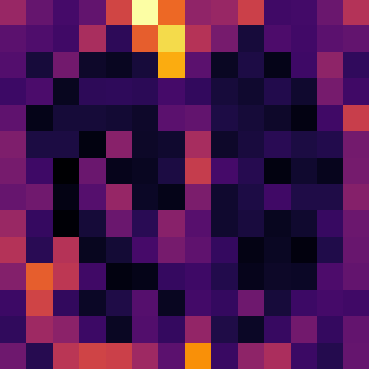
\includegraphics[width=2cm]{attention_ViT_T16-Derma_SSL_Dino_headless_plantvillage.png} & 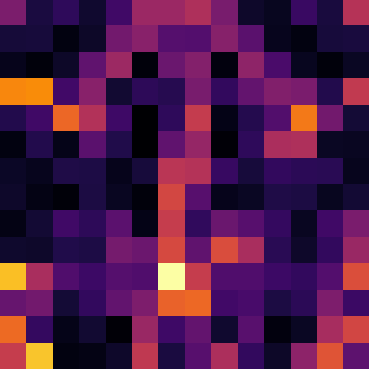
\includegraphics[width=2cm]{attention_ViT_T16-Derma_SSL_Dino_headless_plantdoc.png} & 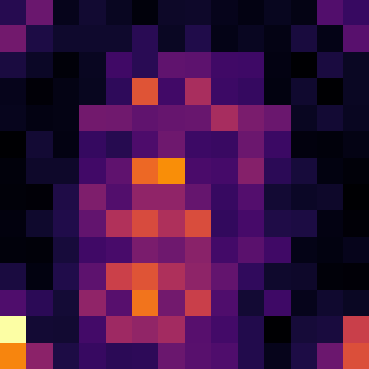
\includegraphics[width=2cm]{attention_ViT_T16-Derma_SSL_Dino_headless_ham10000.png} & 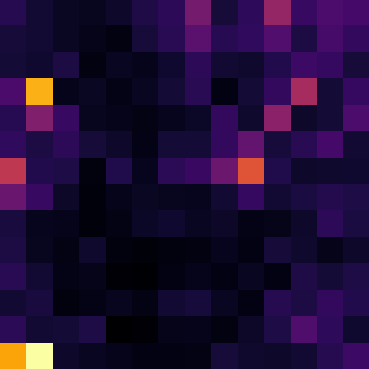
\includegraphics[width=2cm]{attention_ViT_T16-Derma_SSL_Dino_headless_fitzpatrick17k.png} \\
    \end{tabular}
}{icon_8.png}

\slidedefault{Model attention}{
    \framesubtitle{Plant}
    \begin{tabular}{c c c c c}
        \multicolumn{4}{l}{The plant model seems to depict the main vein} \\
        \\
        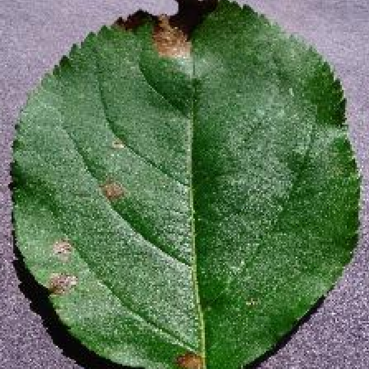
\includegraphics[width=2cm]{attention_input_plantvillage.png} & 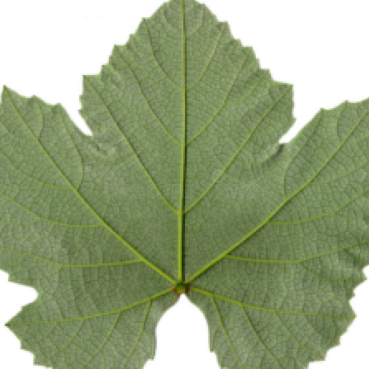
\includegraphics[width=2cm]{attention_input_plantdoc.png} & 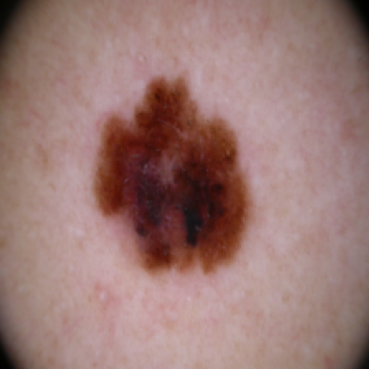
\includegraphics[width=2cm]{attention_input_ham10000.png} & 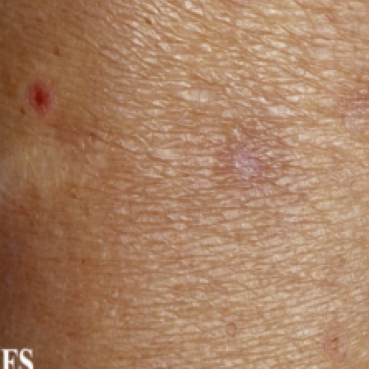
\includegraphics[width=2cm]{attention_input_fitzpatrick17k.png} \\
        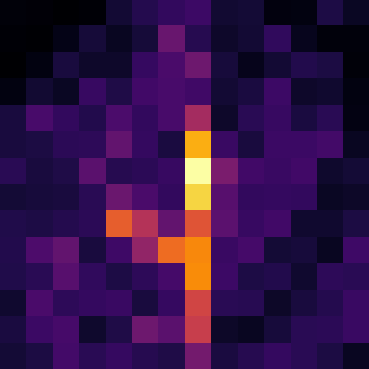
\includegraphics[width=2cm]{attention_ViT_T16-Plant_SSL_Dino_headless_plantvillage.png} & 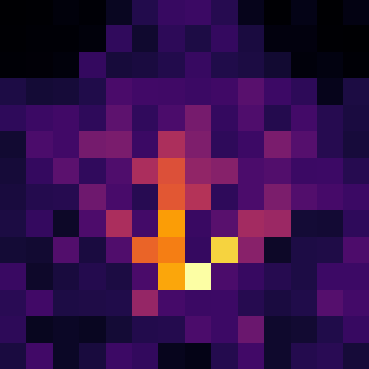
\includegraphics[width=2cm]{attention_ViT_T16-Plant_SSL_Dino_headless_plantdoc.png} & \includegraphics[width=2cm]{attention_ViT_T16-Plant_SSL_Dino_headless_ham10000.png} & \includegraphics[width=2cm]{attention_ViT_T16-Plant_SSL_Dino_headless_fitzpatrick17k.png} \\
    \end{tabular}
}{icon_8.png}

\slidedefault{Evaluation results}{
    \framesubtitle{Resnet50}
    \includegraphics[width=1\textwidth]{spider_resnet50.png}
    Average F1-score from the Resnet50 results
}{icon_10.png}

\slidedefault{Evaluation results}{
    \framesubtitle{Vision transformer}
    \includegraphics[width=1\textwidth]{spider_vit_t16.png}
    Average F1-score from the vision transformer results
}{icon_10.png}

\slidedefault{Subsampling results}{
    \framesubtitle{Overview HAM10000}
    \includegraphics[width=1\textwidth]{lines_ham10000_ViT_T16.png}
    Average F1-score with limited samples per class
}{icon_17.png}

\slidedefault{Subsampling results}{
    \framesubtitle{Training HAM10000}
    \includegraphics[width=1\textwidth]{training_ham10000_ViT_T16_Derma_100.png}
    Training set is fully memorized
}{icon_17.png}

% Consequence would be regularization, right?

\slidedefault{Class comparison}{
    \framesubtitle{HAM10000}
    \begin{tabular}{c c}
        \includegraphics[width=4cm]{confusion_matrix_ham10000_ViT_T16_plant.png} & \includegraphics[width=4cm]{confusion_matrix_ham10000_ViT_T16_imagenet.png} \\
        \\
    \end{tabular}
    Similarity of the confusion matrices of plant and ImageNet
}{icon_15.png}

\slidedefault{Experiments}{
    \framesubtitle{Fine-tuning multiple layers}
    \includegraphics[width=1\textwidth]{fine_tuning_half.png}
    Fine-tuning multiple layers
}{icon_12.png}

% \begin{itemize}
%     \item ???
%     \item ???
% \end{itemize}

%TODO loss curves
\slidedefault{Fine-tuning results}{}{icon_2.png}

%TODO matrix

% \slidedefault{Teacher / student}{}{icon_2.png}
\slidedefault{Teacher / student}{}{icon_2.png}

% \section{Fundamental problem}
% \section{Basic idea}
% \section{Related work}
% \framesubtitle{This is a subtitle}
% \subsection{Related work subject \#1}
% \begin{frame}{Related work}
%     \framesubtitle{Related work subject \#1}
%     \begin{columns}[T]
%         \column{0.5\textwidth}
%             column left
%         \column{0.5\textwidth}
%             column right
%     \end{columns}
%     \note{
%         Notes....
%     }
% \end{frame}

\begin{frame}{Questions and answers}
    \begin{center}
    {\fontsize{40}{50}\selectfont Thank You! \\[10pt] Q \& A}
    \end{center}
\end{frame}

%% REFERENCES
% allowframebreaks: creates multiple slides if it is to long for one

% image: Flaticon.com
\begin{frame}[allowframebreaks]{References}
    \begin{thebibliography}{}
        \setbeamertemplate{bibliography item}[book]
        \bibitem{DeepLearning}
        Goodfellow, Ian, Yoshua Bengio, and Aaron Courville.
        \newblock \emph{Deep Learning}.
        \newblock MIT Press, 2016.
        
        \setbeamertemplate{bibliography item}[article]
        \bibitem{FaceNet}
        Schroff, Florian, Dmitry Kalenichenko, and James Philbin.
        \newblock \emph{FaceNet: A Unified Embedding for Face Recognition and Clustering}, 2015.
        \newblock \url{https://arxiv.org/abs/1503.03832}
        
        \setbeamertemplate{bibliography item}[online]
        \bibitem{DCASE}
        Dekkers, Lauwereins, Thoen et al.
        \newblock \emph{DCASE Challenge 2018 Task 5}, 2018.
        \newblock \url{http://dcase.community/challenge2018/task-monitoring-domestic-activities}
    \end{thebibliography}
\end{frame}

%% APPENDIX
% \appendix

%%%% BACKUP
\begin{frame}{Backup Slides}
	\framesubtitle{backup slides}
	Backup!
\end{frame}

%%
\end{document}
